
\documentclass[12pt,a4paper]{article}

%% Language and font encodings
\usepackage[french, english]{babel}

\usepackage[utf8x]{inputenc}
\usepackage[T1]{fontenc}
\usepackage{footnote}
\usepackage{pgfplots}
\usepackage{tikz}
\usepackage{multicol}
\usepackage{diagbox}
\usepackage{float}
\usepackage{lastpage}
\usepackage{array}
\usepackage{fancyhdr}
\usepackage[english]{fancyref}
\usepackage[UKenglish]{datetime}
\usepackage{pdfpages}
%\usepackage{todonotes}
\usepackage{placeins}
%% Sets page size and margins
\usepackage[a4paper,top=3cm,bottom=2cm,left=3cm,right=3cm,marginparwidth=1.75cm]{geometry}
\pgfplotsset{width=10cm,compat=1.9}
\setlength{\columnsep}{0.3cm}
\pagestyle{fancy}
\cfoot{Page \thepage \hspace{1pt} of \pageref{LastPage}}

%% Useful packages
\usepackage{amsmath}
\usepackage{graphicx}
\definecolor{titlepagecolor}{cmyk}{0,0,0,0}
\definecolor{namecolor}{cmyk}{1,1,1,1}
\usepackage{subcaption}
\usepackage[colorinlistoftodos]{todonotes}
\usepackage[colorlinks=true, allcolors=black]{hyperref}
\usepackage{wrapfig}
\usepackage{listings}
\renewcommand{\thefigure}{\arabic{section}.\arabic{figure}}
%\renewcommand{\thetable}{\arabic{section}.\arabic{figure}}

\definecolor{mGreen}{rgb}{0,0.6,0}
\definecolor{mGray}{rgb}{0.5,0.5,0.5}
\definecolor{mPurple}{rgb}{0.58,0,0.82}
\definecolor{backgroundColour}{rgb}{0.99,0.99,0.99}

\lstdefinestyle{CStyle}{
	backgroundcolor=\color{backgroundColour},   
	commentstyle=\color{mGreen},
	keywordstyle=\color{magenta},
	numberstyle=\tiny\color{mGray},
	stringstyle=\color{mPurple},
	basicstyle=\footnotesize,
	breakatwhitespace=false,         
	breaklines=true,                 
	captionpos=b,                    
	keepspaces=true,                 
	numbers=left,                    
	numbersep=5pt,                  
	showspaces=false,                
	showstringspaces=false,
	showtabs=false,                  
	tabsize=2,
	language=C
}
\lstdefinestyle{PyStyle}{
	backgroundcolor=\color{backgroundColour},   
	commentstyle=\color{mGreen},
	keywordstyle=\color{magenta},
	numberstyle=\tiny\color{mGray},
	stringstyle=\color{mPurple},
	basicstyle=\footnotesize,
	breakatwhitespace=false,         
	breaklines=true,                 
	captionpos=b,                    
	keepspaces=true,                 
	numbers=left,                    
	numbersep=5pt,                  
	showspaces=false,                
	showstringspaces=false,
	showtabs=false,                  
	tabsize=2,
	language=Python
}
\lstset{
	basicstyle=\ttfamily,
	columns=fullflexible,
	showstringspaces=false,
	commentstyle=\color{gray}\upshape
}

\lstdefinelanguage{XML}
{
	morestring=[b]",
	morestring=[s]{>}{<},
	morecomment=[s]{<?}{?>},
	numberstyle=\tiny\color{mGray},       
	breaklines=true, 
	numbers=left,            
	numbersep=5pt,       
	identifierstyle=\color{mGreen},
	keywordstyle=\color{magenta},
	morekeywords={xmlns,version,type}% list your attributes here
}
%\usepackage{natbib}
\pagestyle{fancy}
\title{Development and study of ailerons vs. twisting wing}
\author{\large{Negretto Didier Chérubin, MT-MA-3}}
\makeindex

\begin{document}
	\date{\today}
\begin{titlepage}
\hspace{+2.8cm} %defines the geometry for the titlepage
\pagecolor{titlepagecolor}
\noindent

\includegraphics[width=8cm]{fig/EPFL_Logo_Digital_RGB_PROD.jpg}\\[-1em]
\color{black}
\hspace{+3.5cm}
\makebox[3pt][l]{\rule{8 cm}{1pt}}
\par
\noindent
\hspace{+4.5cm}
\textbf{\Large \textsf{Biorobotics laboratory}}\\
\vspace{0.5cm}
\hspace{-3.5cm}
	%\begin{figure}[H]
    %	\centering
		%\includegraphics[width=12 cm]{fig/frontpage_1.pdf}
		%\includegraphics[width=0.48\linewidth]{fig_pos/FS}
		%\raisebox{-5cm}{\reflectbox{\includegraphics[width=0.48\linewidth]{fig_pos/BS}}}
%					\includegraphics[width=0.49\linewidth]{fig_pos/BS}
%		\reflectbox{\includegraphics[width=0.49\linewidth]{fig_pos/BS}}
	%\end{figure}

\vfill


\hspace{+0.5cm}
{\huge \huge \textsf{MOUSE TREADMILL CONTROL}}

\vskip\baselineskip
\noindent
\hspace{+3.5cm}
{\textsf{\today}
\vskip\baselineskip
\noindent
\hspace{+3.5cm}
{\textsf{By \textbf{\Large{Didier Chérubin Negretto} }}}
\vskip\baselineskip
\noindent
\hspace{+3.5cm}
{\textsf{Professor: \large\textbf{Auke Ijspeert}}}
\vskip\baselineskip
\noindent
\hspace{+3.5cm}
{\textsf{Assistant 1:\textbf{Shravan Tata Ramalingasetty} }}
}
\end{titlepage}

\restoregeometry % restores the geometry
\nopagecolor% Use this to restore the color pages to white
\begin{center}
\chead{\textit{\textbf{Mouse treadmill control}}}
%\newpage
\textbf{\Large{Semester project description}}\\
\end{center}
\begin{multicols}{2}
[]

\paragraph{Objectives and preliminary considerations} 
\lfoot{\today}
\rfoot{Biorobotics laboratory}
The project consists of designing and manufacturing of a lightweight mechanism to improve roll authority at low angles of attack. After that the mechanism is tested and conclusions, with respect to the existing mechanism are drawn.
A drone with morphing wings was designed and manufactured in the months before this project. The drone has wings with artificial overlapping feathers at the wing tip, which are used for roll control. The roll rate obtained at low angles of attack is too low to grant the desired high manoeuvrability as shown by \cite{ref6} for a similar roll control strategy. In the first part of the project different methods are taken into account: ailerons, which are used in the aircraft industry and wing twisting, which is inspired by birds \cite{bird}. Those methods are simulated on XFLR5 (using VLM and 3D-Panels), after which wing twisting is chosen for implementation and testing. Wing twisting has many advantages compared to ailerons: higher roll moment \cite{real_plane} and higher lift to drag ratio \cite{ref3}. On the other hand this technique is less used in industry and leads to an increased weight of the drone. 
%\begin{figure}[H]
%	\includegraphics[width=0.8\linewidth]{fig_des/exp_setup.jpg}
%	\caption{Photo taken during the wind tunnel test, with a symmetric backward sweep configuration. }\label{fig:wind}
%\end{figure}
\paragraph{Mechanism design}
 A weight of less than 20 [$g$] is required as well as the interoperability with the pre-existing folding mechanism. Four different designs are taken into account (partial twisting, flexible components, cylindrical element and ball joints). In the end the design consisting of a lever actuated by a servo (ball joints) is chosen for implementation. This design is simple and can generate the required roll (roll control power over 2 [$\frac{\partial C_r}{\partial rad}$] for $\alpha \leq 8^\circ$) at low angles of attack, solving the initial problem. The folding angle $\phi$ is defined as the sum of the angles compared to normal sweep on the two sides. 
\paragraph{Testing and results}
\begin{figure}[H]
	\centering
	%\includegraphics[width=1.2\linewidth]{fig_des/fin_comp}
	%\includegraphics[width=\linewidth]{fig_sim/fin_comp}
	\caption{Roll coefficient as a function of the angle of attack for different values of twisting and folding angles. Schematics of folding configurations are added. }\label{fig:tw_vs_fold_bar}
\end{figure}
The third part consists of testing the drone in the wind tunnel at different angles of attack (from 0$^\circ$ to 28$^\circ$ with steps of 4$^\circ$), at three different twisting angles (0$^\circ$, 5$^\circ$ and 10$^\circ$), and with three possible wing shapes to take into account the effect of folding. Most of roll is generated with twisting at low angles of attack ($\alpha<8^\circ$), while at high angles folding has a greater impact (see figure \ref{fig:tw_vs_fold_bar}).
\paragraph{Roll control and cost}
Finally a roll control algorithm for folding and twisting wing drones is presented.  This is one of the most important accomplishments of this report since a study of different roll control methods on the same platform is, at the best of our knowledge, absent in literature. The cost of such a setup is discussed as well. This cost is very low, mainly due to the weight of the mechanism and to the energy consumption since the loss of aerodynamic performances during roll is small ($C_d$ +38,98\%), compared to the roll achieved ($C_r = 0.4519$ [ ]).

\end{multicols}

\clearpage
\lfoot{ }
\rfoot{ }
\chead{ }
%\begin{abstract}

%\end{abstract}

\pagestyle{plain}
\clearpage

\tableofcontents
\clearpage
\pagestyle{fancy}
\section{Introduction}\label{sec:intro}
In this section the main objectives and the state of the art for the project are presented as well as the overall structure of this report.
\subsection{Motivation}
\begin{wrapfigure}{L}{0.42\textwidth}
	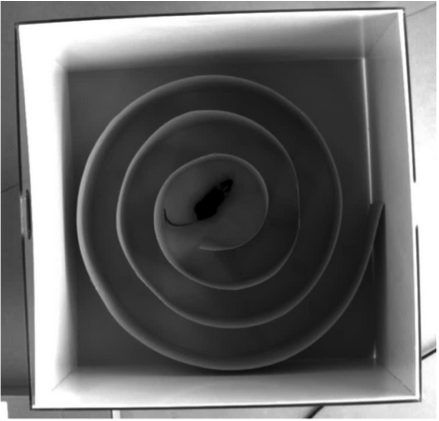
\includegraphics[width=\linewidth]{fig/OleSetup.png}
	\caption{The experimental setup used in \cite{Ole}.}\label{fig:OleSetup}
	\vspace{-3.0 cm}
\end{wrapfigure}
The studies on mammal locomotion have driven more and more attention over the years, and especially experiments on mice, such as \cite{Ole}, have enhanced our understanding of the neuronal circuits that enable locomotion. The experimental setup in \cite{Ole}, on the other hand, is quite rudimental. As shown in \ref{fig:OleSetup} it only consist in a spiral maze made out cardboard. This setup comes with some advantages such as:
\begin{itemize}
	\item Low price
	\item Simple to implement and use
	\item Untrained mice can be employed
	\item Free moving mouse
\end{itemize}
As well as some disadvantages:
\begin{itemize}
	\item Impossibility to analyse the mouse gait
	\item The mouse movements can't be imposed
\end{itemize}
To asses these issues a new design is needed for conducting such experiments. The new platform needs to allow the control on the walking surface on which the mouse is standing in such a way that a specific speed profile can be imposed to the mouse. Moreover it must be possible to analyse the mouse gait using cameras. \\
For the new design inspiration is taken from some existing solutions on the market. 
\subsection{Requirements}
First the mechanical requirements are discussed and stated. Table \ref{tab:Requirements} summarizes them.
\begin{table}[H]
	\centering
	\begin{tabular}{l||c|r} 
		\textbf{Description}&\textbf{Value}  &\textbf{Unit}  \\ 
		\hline
		\hline 
		Dimensions of the moving surface & 0.5 & $[m^2]$ \\ 
		\hline 
		Course & $\infty$  & $[m]$  \\ 
		\hline 
		Maximum speed & 3 & $[\frac{m}{s}]$ \\ 
		\hline 
		Maximum acceleration & 2 & $[\frac{m}{s^2}]$  \\ 
		\hline 
		Position resolution & 0.01 & $[m]$  \\ 
		\hline 
		Speed resolution & 0.02  & $[\frac{m}{s}]$  \\ 
		\hline 
		Maximum weight & 0.1  & $[kg]$  \\  
		\hline 
		Mounting time for 1 person & 30 & $[min]$  \\
		\hline 
		Maximum weight of the mouse & 40  & $[g]$ \\
		\hline 
		Length of common experiment (distance, time) & (20, 600)  & ($[m]$,$[s]$)  \\
	\end{tabular} 
	\caption{Summary of the requirements for the mouse treadmill platform.}
	\label{tab:Requirements}
\end{table}
The functional requirements are listed as well:
\begin{itemize}
	\item \textbf{Closed-loop control} Once a 2D speed setpoint is chosen the speed of the surface needs to be measured and the motor control signal need to be adjusted automatically to reach the desired setpoint. 
	\item \textbf{Speed routines} The user can define a speed routine, which needs to be executed by the treadmill. The speed routine consist in a list of 2D speed setpoints and the time interval during which the machine should execute them.
	\item \textbf{User interface} The user can use a Graphical user interface (GUI) on a computer to be able to use the mouse treadmill. This interface informs the user if the sensors are correctly connected and initialized, and it should give a live update of the treadmill speed.
	\item \textbf{Data logging} The user can save the data sent by the treadmill during the experiment for future uses. 
	\item \textbf{Expandability of the system} The user can easily expand the system with other controllers to have other features, than the ones listed above.
\end{itemize}

\subsection{Structure of the report}
This report is structured as follows: an introduction is given in section \ref{sec:intro}, the system architecture and communication are explained in \ref{sec:archi}. Section \ref{sec:design}, describes the design decisions and the components choices made .Section \ref{sec:control} describes the control strategy and shows some preliminary responses.
Finally in section \ref{sec:conc} the conclusion of the project is given. The code, code documentation as well as the data-sheets of the components are annexed.

\section{System architecture and communication} \label{sec:archi}
In this section the architecture and the communication are explained and detailed.
\subsection{System architecture}
In this section the architecture and interfaces between the different components of the machine are detailed.

\section{Design choices}\label{sec:design}
In this section the design choices are explained and justified. First the choice of the board is analysed, then the sensors and finally the calculations for the motor dimensioning are shown.
\subsection{Board}
For the board choice different types are taken into account:
\begin{itemize}
	\item \textbf{Single board computer}: In this category the raspberry pi and the odroid are taken into consideration. These boards offer powerful computers, which can be running operating systems such as Linux or Windows, which makes them interesting. Unfortunately they can't provide any accurate timing,  which is needed for the motor control and PWM generation.
	\item \textbf{Evaluation boards}: In this category the STM32 nucleo boards as well as the arduino boards can be found. These boards allow proper timing of the signals and accurate PWM generation, but on the other hand a computer is needed for plotting and storing the data, which can't be done locally on the board due to memory restrictions and limited resources on the board.
\end{itemize}
Due to the constraints in the system the second category is consider for implementation, the STM32L476RG board is taken for the system. Table \ref{tab:board} summarizes the features of the board.
\begin{table}[H]
	\centering
	\begin{tabular}{l||c|r} 
		\textbf{Description}&\textbf{Value}  &\textbf{Unit}  \\ 
		\hline
		\hline 
		Architecture & ARM-Cortex 32-bit with FPU & $-$ \\ 
		\hline 
		Clock frequency & 80  & $[MHz]$  \\ 
		\hline 
		Flash memory & 1 & $[MB]$ \\ 
		\hline 
		RAM memory & 128 & $[KB]$  \\ 
		\hline 
		I2C interfaces & 3 & $-$  \\ 
		\hline 
		USART interfaces & 5  & $-$  \\ 
		\hline 
		SPI interfaces & 3  & $-$  \\  
		\hline 
		DMA controller & 14 & $-$  \\
		\hline
		Cost & 20.58 &$[CHF]$
	\end{tabular} 
	\caption{STM32L476RG main features.}
	\label{tab:board}
\end{table}
One of the most important feature of the board is the DMA, which enhances the performances of the CPU. The DMA is used for the UART communication with the computer. This technique frees the CPU from waiting for the UART communication to be finished, so that it can spend more time on other activities. This same solution can be, in principle, adopted for the SPI communication if a standard SPI is used. Unfortunately the timing diagrams for the sensors are not standard, thus some time needs to be "wasted" by the processor so that the sensors can keep up with the communication.
Other interesting features are: the big flash memory, the good RAM memory and the low cost. One drawback is that dynamic memory allocation is not possible in such an small system to prevent stack overflow and problems during run time. This is why the size of the speed routine is limited to a given number of points.
Finally the multiple serial interfaces allow the possibility to expand the system to a bigger one with more controllers involved.

\subsection{Communication}
\begin{wrapfigure}{R}{0.42\textwidth}
	
\includegraphics[width=\linewidth]{fig/MAVLink_logo.png}
	\caption{MAVLink logo}\label{fig:MAVLink_logo}
\end{wrapfigure}
For the communication with the computer the UART protocol is chosen. This choice is almost mandatory since most boards are provided with an UART to USB interface and a mini-USB connector. The STM32L476RG is no exception to this rule.

Since the system needs to be expanded for future more complex experiments some thought is put in the choice of the messaging protocol to allow this key feature.
The best solution found is MAVLink. "MAVLink is a very lightweight messaging protocol for communicating with drones"\cite{mavlink}, one can say that the mouse treadmill is not meant to fly around, but this messaging protocol is flexible enough to be adapted to the mouse treadmill.
More precisely a dialect is described in \ref{app:mavlink}, and summarized in table \ref{tab:msg}. Thanks to the description file it is possible to generate libraries in different programming languages (C, Python, Java, ...) and if in the future a new message is required a additional definition can be added to the file and the libraries can be regenerated.

Despite the light weight MAVLink comes with some interesting features, such is high reliability (detects packets drops and corruption), high efficiency (only 14-bits of overhead), it can also allow up to 255 concurrent systems on the network.

\begin{table}[H]
	\centering
	\begin{tabular}{l||p{3cm}|l|l} 
		\textbf{Name} &\textbf{Description} &\textbf{Sender} &\textbf{Receiver}\\ 
		\hline
		\hline 
		HEARTBEAT &Verifies communication& STM32 & PC \\ 
		\hline 
		SPEED\_INFO &Measured speed  & STM32 & PC \\ 
		\hline 
		SPEED\_SETPOINT & Speed setpoint & PC & STM32 \\ 
		\hline 
		MODE\_SELECTION & Changes mode & PC & STM32  \\ 
		\hline 
		MOTOR\_SETPOINT & Up time of PWM duty cycle & STM32 & PC  \\ 
		\hline 
		POINT\_LOADED & Acknowledge for routine point loaded  & STM32 & PC  \\ 
		\hline 
		POINT & Information for one point of the routine  & PC & STM32  \\  
		\hline 
		ERROR & Error message & STM32 & PC  \\
		\hline
		RAW\_SENSOR & Raw sensor values & STM32 & PC \\
	\end{tabular} 
	\caption{List and description of the MAVLink messages.}
	\label{tab:msg}
\end{table}


\subsection{Sensor}
For sensing the speed of the wheel a contactless solution is chosen. To have achive this goal a optical gaming mouse sensor is taken. Nevertheless the sensor need to come mounted on a PCB with a simple interface to reduce the time needed to design and manufacture the machine. 

\subsection{Motor}
To properly dimension the motors these assumptions are taken:
\begin{enumerate}
	\item $\eta = 1$ No losses in wheel-sphere coupling
	\item No slip of the wheel on the sphere
	\item Hollow sphere
	\item Flat disk
\end{enumerate}

The data given are:
\begin{itemize}
	\item $m_s$ mass of the sphere
	\item $r_s$ radius of the sphere
	\item $m_w$ mass of the wheel
	\item $r_w$ radius of the wheel
	\item $M_{max}$ maximum torque provided by the motor-gearbox 
	\item $\omega_{max}$ maximum angular speed of the motor-gearbox
	\item $J_m$ inertia of the rotor
\end{itemize}
It is therefore possible to estimate the maximum continuous  acceleration and speed of the sphere.

\section{Control} \label{sec:control}

\section{Conclusion} \label{sec:conc}



\clearpage
\lhead{ }
\begin{thebibliography}{100}
	
	\bibitem{Ole}Jared M. Cregg, Roberto Leiras, Alexia Montalant, Ian R. Wickersham, and Ole Kiehn, \textit{Brainstem Neurons that Command Left/Right Locomotor Asymmetries} 
	\bibitem{mavlink} MAVLink Developer Guide, \textit{https://mavlink.io/en/}
	
	\bibitem{sar} Robin R. Murphy, Eric Steimle et al. \textit{Cooperative Use of Unmanned Sea Surface and Micro Aerial Vehicles at Hurricane Wilma},Journal of Field Robotics,2008
	\bibitem{eco}     Kenzo Nonami, Farid Kendoul, Satoshi Suzuki, Wei Wang, Daisuke Nakazawa,\textit{Autonomous Flying Robots}, Springer, 2010.
	\bibitem{roll} G. Sachs, \textit{What Can Be Learned from Unique Lateral-Directional Dynamics Properties of Birds for Mini-Aircraft}, Atmospheric Flight Mechanics Conference and Exhibit, 2007
	%\bibitem{ref1} Onur Bilgen, Kevin B. Kochersberger, and Daniel J. Inman, \textit{Novel, Bidirectional, Variable-Camber Airfoil via Macro-Fiber Composite Actuators}, Journal of aircraft Vol. 47, No. 1, January–February 2010.
	\bibitem{real_plane} R. Pecora, F. Amoroso, and L. Lecce, \textit{Effectiveness of Wing Twist Morphing in Roll Control}, Journal of aircraft Vol. 49, No. 6, November–December 2012
	\bibitem{ref3} Osgar John Ohanian III, Christopher Hickling, Brandon Stiltner, Etan D. Karni, \textit{Piezoelectric Morphing versus Servo-Actuated MAV Control Surfaces}, 53rd AIAA/ASME/ASCE/AHS/ASC Structures, Structural Dynamics and Materials Conference, 2012
	\bibitem{ref4} Helen M. Garcia , Mujahid Abdulrahim and Rick Lind, \textit{Roll control for a micro air vehicle using active wing morphing}, AIAA Guidance, Navigation, and Control Conference and Exhibit, 2003
	\bibitem{ref5} Mujahid Abdulrahim, Helen Garcia, and Rick Lind, \textit{Flight Characteristics of Shaping the Membrane Wing of a Micro Air Vehicle}, Journal of aircraft Vol. 42, No. 1, January–February 2005
	\bibitem{ref6} M. Di Luca, S. Mintchev, G. Heitz, F. Noca and D. Floreano, \textit{Bioinspired morphing wings for extended flight envelope and roll control of small drones}, Interface Focus 7, 2017
	\bibitem{urb_env} William E. Green and Paul Y. Oh, \textit{A Hybrid MAV for Ingress and Egress of Urban Environments}, IEEE transactions on robotics, 2009
	\bibitem{twist} Bret Stanford, Mujahid Abdulrahim, Rick Lind, and Peter Ifju, \textit{Actuation for Roll Control of a Micro Air Vehicle}, Journal of aircraft,  2007
	\bibitem{rev} Juan Carlos Gomez and Ephrahim Garcia, \textit{Morphing unmanned aerial vehicles}, Smart materials and structures, 2011.
	\bibitem{book} E.L. Houghton, P.W. Carpenter, Steven H. Collicott and Daniel T. Valentine, \textit{Aerodynamics for engineering students}, Seventh edition.
	\bibitem{fire} Pero Skorput, Sadko Mandzuka, Hrvoje Vojvodic, \textit{The Use of Unmanned Aerial Vehicles for Forest Fire Monitoring }, 58th International Symposium ELMAR, 2016
	\bibitem{city} David Gallacher, \textit{Drone Applications for Environmental Management in Urban Spaces: A Review}, International Journal of Sustainable Land Use and Urban Planning, 2016
	\bibitem{disaster} Ludovic Apvrille, Tullio Tanzi, and Jean-Luc Dugelay \textit{Autonomous Drones for Assisting Rescue Services within the context of Natural Disasters}, XXXIth URSI General Assembly and Scientific Symposium, 2014
\end{thebibliography}
\bibliographystyle{plainnat}
\listoffigures
\listoftables
\appendix
\section{MAVLink dialect description file}\label{app:mavlink}
\lstinputlisting[language=XML]{../mouse.xml}
\section{Code for STM32 NUCLEO 64 board}
\subsection{Main}
\lstinputlisting[style=CStyle]{../MouseTreadmillSTM32Project/Core/Inc/main.h}
\lstinputlisting[style=CStyle]{../MouseTreadmillSTM32Project/Core/Src/main.c}
\subsection{Treadmill driver}
\lstinputlisting[style=CStyle]{../CodeSTM32/src/mouseDriver.c}
\lstinputlisting[style=CStyle]{../CodeSTM32/src/mouseDriver.h}
\subsection{Sensor driver}
\lstinputlisting[style=CStyle]{../CodeSTM32/src/sensorDriver.c}
\lstinputlisting[style=CStyle]{../CodeSTM32/src/sensorDriver.h}
\subsection{Code for unit tests}
\lstinputlisting[style=CStyle]{../CodeSTM32/test/display.h}
\lstinputlisting[style=CStyle]{../CodeSTM32/test/main.c}
\lstinputlisting[style=CStyle]{../CodeSTM32/test/mock_mouseDriver.h}
\lstinputlisting[style=CStyle]{../CodeSTM32/test/mock_sensorDriver.h}
\lstinputlisting[style=CStyle]{../CodeSTM32/test/test_mouseDriver.h}
\lstinputlisting[style=CStyle]{../CodeSTM32/test/test_sensorDriver.h}
\lstinputlisting[style=CStyle]{../CodeSTM32/test/test_mouseDriver.c}
\lstinputlisting[style=CStyle]{../CodeSTM32/test/test_sensorDriver.c}
\subsection{Build script}
\lstinputlisting[style=CStyle]{../CodeSTM32/src/build.sh}

\section{Code for PC}
\subsection{GUI}
\lstinputlisting[style=PyStyle]{../MouseTreadmillPC/python/mouseController.py}
\subsection{Routine example}
\lstinputlisting[style=PyStyle]{../MouseTreadmillPC/python/routine.py}
\subsection{Sensor data-sheet}
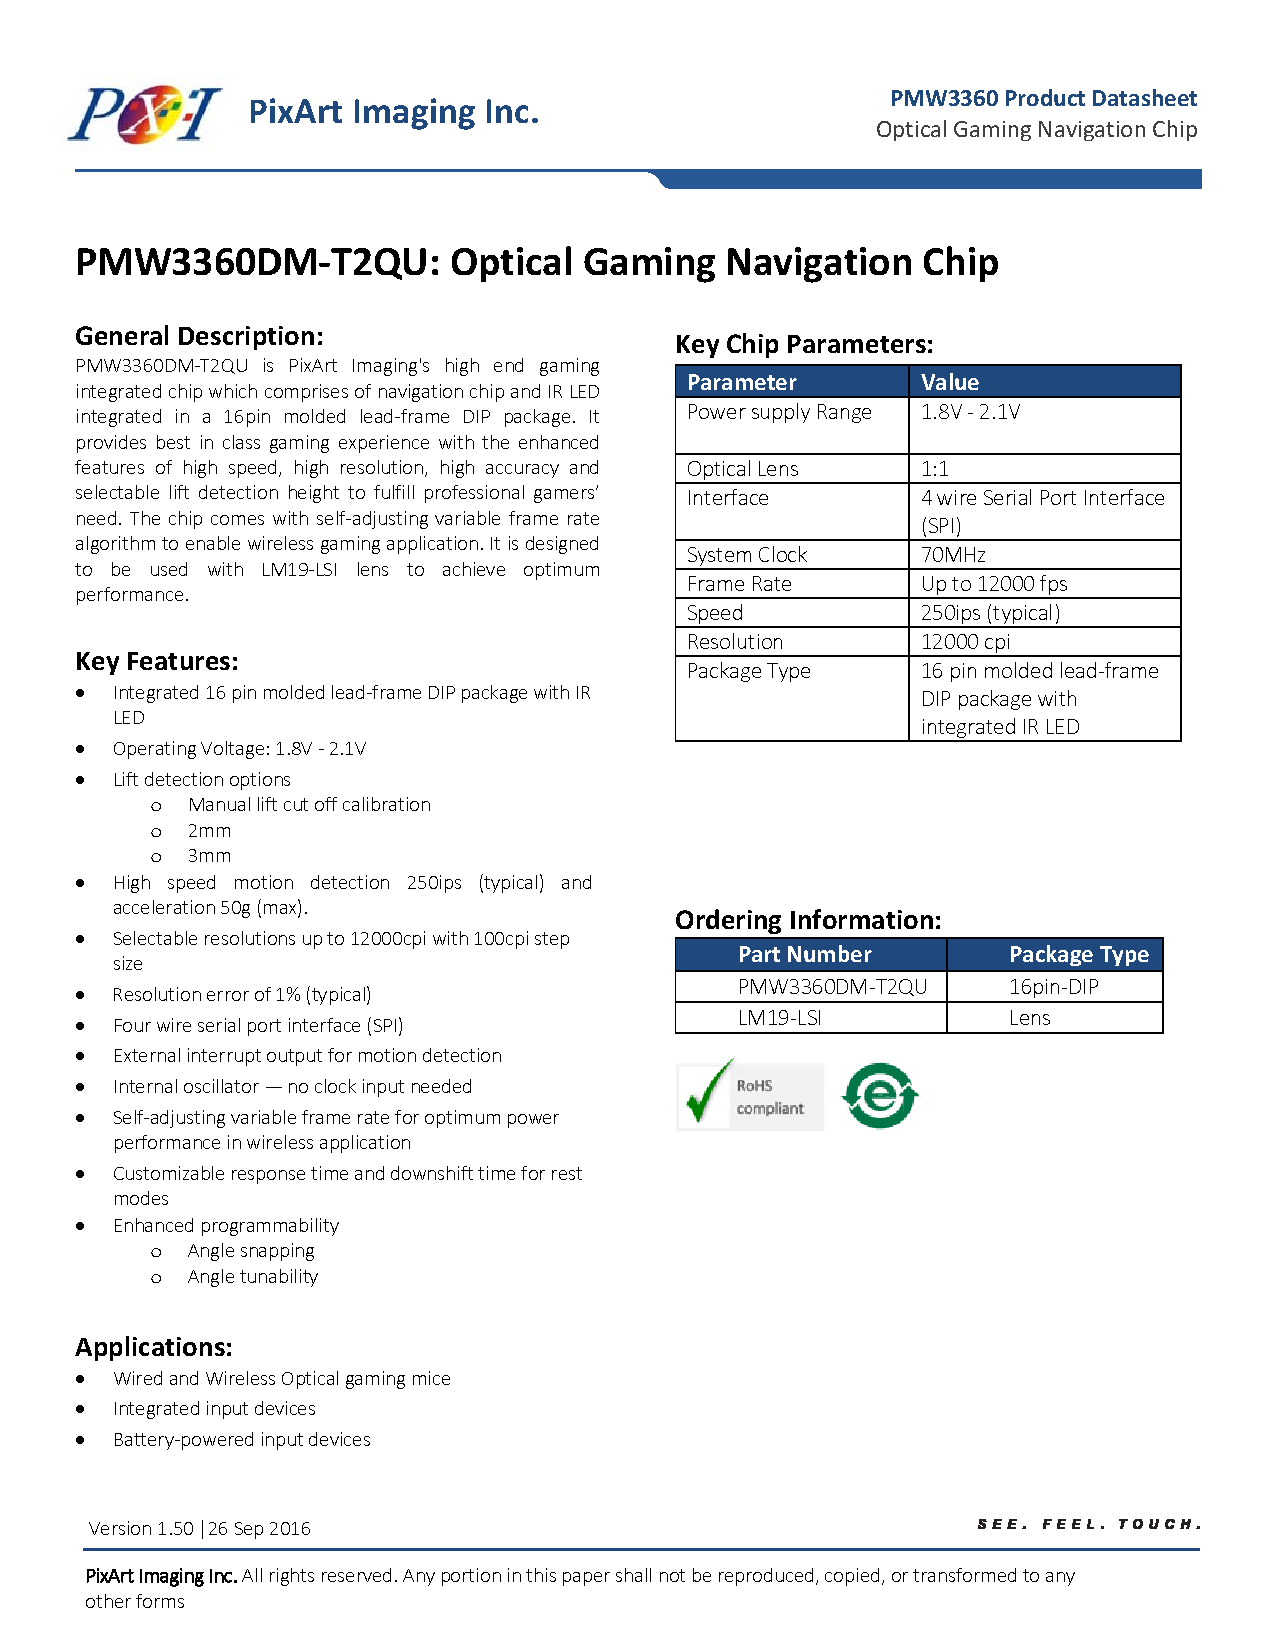
\includepdf[pages=-]{../resources/sensorDatasheet.pdf}
%\let\mypdfximage\pdfximage\def\pdfximage{\immediate\mypdfximage}\documentclass[twoside]{book}

%% moved from doxygen.sty due to workaround for LaTex 2019 version and unmaintained tabu package
\usepackage{ifthen}
\ifx\requestedLaTeXdate\undefined
\usepackage{array}
\else
\usepackage{array}[=2016-10-06]
\fi
%%
% Packages required by doxygen
\usepackage{fixltx2e}
\usepackage{calc}
\usepackage{doxygen}
\usepackage{graphicx}
\usepackage[utf8]{inputenc}
\usepackage{makeidx}
\usepackage{multicol}
\usepackage{multirow}
\PassOptionsToPackage{warn}{textcomp}
\usepackage{textcomp}
\usepackage[nointegrals]{wasysym}
\usepackage[table]{xcolor}
\usepackage{ifpdf,ifxetex}

% Font selection
\usepackage[T1]{fontenc}
\usepackage[scaled=.90]{helvet}
\usepackage{courier}
\usepackage{amssymb}
\usepackage{sectsty}
\renewcommand{\familydefault}{\sfdefault}
\allsectionsfont{%
  \fontseries{bc}\selectfont%
  \color{darkgray}%
}
\renewcommand{\DoxyLabelFont}{%
  \fontseries{bc}\selectfont%
  \color{darkgray}%
}
\newcommand{\+}{\discretionary{\mbox{\scriptsize$\hookleftarrow$}}{}{}}

% Arguments of doxygenemoji:
% 1) ':<text>:' form of the emoji, already "LaTeX"-escaped
% 2) file with the name of the emoji without the .png extension
% in case image exist use this otherwise use the ':<text>:' form
\newcommand{\doxygenemoji}[2]{%
  \IfFileExists{./#2.png}{\raisebox{-0.1em}{\includegraphics[height=0.9em]{./#2.png}}}{#1}%
}
% Page & text layout
\usepackage{geometry}
\geometry{%
  a4paper,%
  top=2.5cm,%
  bottom=2.5cm,%
  left=2.5cm,%
  right=2.5cm%
}
\tolerance=750
\hfuzz=15pt
\hbadness=750
\setlength{\emergencystretch}{15pt}
\setlength{\parindent}{0cm}
\newcommand{\doxynormalparskip}{\setlength{\parskip}{3ex plus 2ex minus 2ex}}
\newcommand{\doxytocparskip}{\setlength{\parskip}{1ex plus 0ex minus 0ex}}
\doxynormalparskip
\makeatletter
\renewcommand{\paragraph}{%
  \@startsection{paragraph}{4}{0ex}{-1.0ex}{1.0ex}{%
    \normalfont\normalsize\bfseries\SS@parafont%
  }%
}
\renewcommand{\subparagraph}{%
  \@startsection{subparagraph}{5}{0ex}{-1.0ex}{1.0ex}{%
    \normalfont\normalsize\bfseries\SS@subparafont%
  }%
}
\makeatother

% Headers & footers
\usepackage{fancyhdr}
\pagestyle{fancyplain}
\fancyhead[LE]{\fancyplain{}{\bfseries\thepage}}
\fancyhead[CE]{\fancyplain{}{}}
\fancyhead[RE]{\fancyplain{}{\bfseries\leftmark}}
\fancyhead[LO]{\fancyplain{}{\bfseries\rightmark}}
\fancyhead[CO]{\fancyplain{}{}}
\fancyhead[RO]{\fancyplain{}{\bfseries\thepage}}
\fancyfoot[LE]{\fancyplain{}{}}
\fancyfoot[CE]{\fancyplain{}{}}
\fancyfoot[RE]{\fancyplain{}{\bfseries\scriptsize Generated by Doxygen }}
\fancyfoot[LO]{\fancyplain{}{\bfseries\scriptsize Generated by Doxygen }}
\fancyfoot[CO]{\fancyplain{}{}}
\fancyfoot[RO]{\fancyplain{}{}}
\renewcommand{\footrulewidth}{0.4pt}
\renewcommand{\chaptermark}[1]{%
  \markboth{#1}{}%
}
\renewcommand{\sectionmark}[1]{%
  \markright{\thesection\ #1}%
}

% Indices & bibliography
\usepackage{natbib}
\usepackage[titles]{tocloft}
\setcounter{tocdepth}{3}
\setcounter{secnumdepth}{5}
\makeindex

\usepackage{newunicodechar}
  \newunicodechar{⁻}{${}^{-}$}% Superscript minus
  \newunicodechar{²}{${}^{2}$}% Superscript two
  \newunicodechar{³}{${}^{3}$}% Superscript three

% Hyperlinks (required, but should be loaded last)
\ifpdf
  \usepackage[pdftex,pagebackref=true]{hyperref}
\else
  \ifxetex
    \usepackage[pagebackref=true]{hyperref}
  \else
    \usepackage[ps2pdf,pagebackref=true]{hyperref}
  \fi
\fi

\hypersetup{%
  colorlinks=true,%
  linkcolor=blue,%
  citecolor=blue,%
  unicode%
}

% Custom commands
\newcommand{\clearemptydoublepage}{%
  \newpage{\pagestyle{empty}\cleardoublepage}%
}

\usepackage{caption}
\captionsetup{labelsep=space,justification=centering,font={bf},singlelinecheck=off,skip=4pt,position=top}

\usepackage{etoc}
\etocsettocstyle{\doxytocparskip}{\doxynormalparskip}
\renewcommand{\numberline}[1]{#1~}
%===== C O N T E N T S =====

\begin{document}

% Titlepage & ToC
\hypersetup{pageanchor=false,
             bookmarksnumbered=true,
             pdfencoding=unicode
            }
\pagenumbering{alph}
\begin{titlepage}
\vspace*{7cm}
\begin{center}%
{\Large 3D\+Mouse\+Treadmill \\[1ex]\large 0 }\\
\vspace*{1cm}
{\large Generated by Doxygen 1.8.16}\\
\end{center}
\end{titlepage}
\clearemptydoublepage
\pagenumbering{roman}
\tableofcontents
\clearemptydoublepage
\pagenumbering{arabic}
\hypersetup{pageanchor=true}

%--- Begin generated contents ---
\chapter{File Index}
\doxysection{File List}
Here is a list of all files with brief descriptions\+:\begin{DoxyCompactList}
\item\contentsline{section}{Code S\+T\+M32/\mbox{\hyperlink{mouse_driver_8c}{mouse\+Driver.\+c}} \\*Implementation of the driver for the mouse treadmil project }{\pageref{mouse_driver_8c}}{}
\item\contentsline{section}{Code S\+T\+M32/\mbox{\hyperlink{mouse_driver_8h}{mouse\+Driver.\+h}} \\*Header of the driver for the mouse treadmil project }{\pageref{mouse_driver_8h}}{}
\item\contentsline{section}{Code S\+T\+M32/\mbox{\hyperlink{utils_8h}{utils.\+h}} }{\pageref{utils_8h}}{}
\end{DoxyCompactList}

\chapter{File Documentation}
\hypertarget{mouse_driver_8c}{}\doxysection{Code S\+T\+M32/mouse\+Driver.c File Reference}
\label{mouse_driver_8c}\index{Code STM32/mouseDriver.c@{Code STM32/mouseDriver.c}}


Implementation of the driver for the mouse treadmil project.  


{\ttfamily \#include \char`\"{}mouse\+Driver.\+h\char`\"{}}\newline
\doxysubsection*{Functions}
\begin{DoxyCompactItemize}
\item 
void \mbox{\hyperlink{mouse_driver_8c_a78891a5c0a9ff59e8de3479cef3dd708}{mouse\+Driver\+\_\+init\+Setpoint}} (void)
\item 
void \mbox{\hyperlink{mouse_driver_8c_a399080e7e42aa3cf13e3ae5c6012b731}{mouse\+Driver\+\_\+init\+Time}} (void)
\item 
void \mbox{\hyperlink{mouse_driver_8c_ae21a55ca0039131ed41b563efbb81ddb}{mouse\+Driver\+\_\+init\+Mode}} (void)
\item 
void \mbox{\hyperlink{mouse_driver_8c_ad79b2fdfdd673bb416b89de2bd80927d}{mouse\+Driver\+\_\+get\+Speed\+From\+Sensors}} (void)
\item 
void \mbox{\hyperlink{mouse_driver_8c_aa5609bff60e6d530873ab05bb4dc8e97}{mouse\+Driver\+\_\+set\+Setpoint}} (const mavlink\+\_\+speed\+\_\+setpoint\+\_\+t speed)
\item 
void \mbox{\hyperlink{mouse_driver_8c_a237f0960175af336ca81667d7eb9ef2e}{mouse\+Driver\+\_\+set\+Mode}} (uint8\+\_\+t mode)
\item 
void \mbox{\hyperlink{mouse_driver_8c_a0c549479547ef441f7424ffcbe47de95}{mouse\+Driver\+\_\+send\+Msg}} (uint32\+\_\+t msgid)
\item 
void \mbox{\hyperlink{mouse_driver_8c_a1b501a2d737cbe2636dc76e7d7c9378e}{mouse\+Driver\+\_\+init}} (void)
\begin{DoxyCompactList}\small\item\em Function for initializing the mouse\+Driver. \end{DoxyCompactList}\item 
void \mbox{\hyperlink{mouse_driver_8c_aa7d22c0c2f293182c6197e25e5afb352}{mouse\+Driver\+\_\+set\+Time}} (const uint32\+\_\+t time)
\item 
uint32\+\_\+t \mbox{\hyperlink{mouse_driver_8c_a7908648bbda149bdf1ef821097039684}{mouse\+Driver\+\_\+get\+Time}} (void)
\item 
void \mbox{\hyperlink{mouse_driver_8c_ac6ff4f7ea298a0b01815904468bb29da}{mouse\+Driver\+\_\+read\+Msg}} (const mavlink\+\_\+message\+\_\+t msg)
\item 
void \mbox{\hyperlink{mouse_driver_8c_aaeee34eedb0741b6360ad62ac296cc7e}{mouse\+Driver\+\_\+idle}} (void)
\item 
void \mbox{\hyperlink{mouse_driver_8c_ae148c84e3642827c8d5c34a675d65739}{mouse\+Driver\+\_\+control\+I\+SR}} (void)
\end{DoxyCompactItemize}
\doxysubsection*{Variables}
\begin{DoxyCompactItemize}
\item 
static uint32\+\_\+t \mbox{\hyperlink{mouse_driver_8c_a8e8611558b7ab767b1685a6a350aee53}{actual\+\_\+time}} = 0
\begin{DoxyCompactList}\small\item\em Global variable for time keeping. \end{DoxyCompactList}\item 
static uint8\+\_\+t \mbox{\hyperlink{mouse_driver_8c_a7e2c75a51747c0c5f00ad6c672bc3024}{actual\+\_\+mode}} = M\+O\+U\+S\+E\+\_\+\+M\+O\+D\+E\+\_\+\+S\+T\+OP
\item 
static mavlink\+\_\+speed\+\_\+info\+\_\+t \mbox{\hyperlink{mouse_driver_8c_aa5490b06dbe7d61f3661c8afbd10d317}{actual\+\_\+speed\+\_\+measure}}
\item 
static mavlink\+\_\+speed\+\_\+setpoint\+\_\+t \mbox{\hyperlink{mouse_driver_8c_a2ed2ab5427f1ccd8753023817343ac75}{actual\+\_\+speed\+\_\+setpoint}}
\item 
static mavlink\+\_\+motor\+\_\+setpoint\+\_\+t \mbox{\hyperlink{mouse_driver_8c_ad6abb9303429a23fb0456e5b155cc37c}{actual\+\_\+motor\+\_\+signal}}
\end{DoxyCompactItemize}


\doxysubsection{Detailed Description}
Implementation of the driver for the mouse treadmil project. 

\begin{DoxyAuthor}{Author}
Didier Negretto 
\end{DoxyAuthor}


\doxysubsection{Function Documentation}
\mbox{\Hypertarget{mouse_driver_8c_ae148c84e3642827c8d5c34a675d65739}\label{mouse_driver_8c_ae148c84e3642827c8d5c34a675d65739}} 
\index{mouseDriver.c@{mouseDriver.c}!mouseDriver\_controlISR@{mouseDriver\_controlISR}}
\index{mouseDriver\_controlISR@{mouseDriver\_controlISR}!mouseDriver.c@{mouseDriver.c}}
\doxysubsubsection{\texorpdfstring{mouseDriver\_controlISR()}{mouseDriver\_controlISR()}}
{\footnotesize\ttfamily void mouse\+Driver\+\_\+control\+I\+SR (\begin{DoxyParamCaption}\item[{void}]{ }\end{DoxyParamCaption})}

\mbox{\Hypertarget{mouse_driver_8c_ad79b2fdfdd673bb416b89de2bd80927d}\label{mouse_driver_8c_ad79b2fdfdd673bb416b89de2bd80927d}} 
\index{mouseDriver.c@{mouseDriver.c}!mouseDriver\_getSpeedFromSensors@{mouseDriver\_getSpeedFromSensors}}
\index{mouseDriver\_getSpeedFromSensors@{mouseDriver\_getSpeedFromSensors}!mouseDriver.c@{mouseDriver.c}}
\doxysubsubsection{\texorpdfstring{mouseDriver\_getSpeedFromSensors()}{mouseDriver\_getSpeedFromSensors()}}
{\footnotesize\ttfamily void mouse\+Driver\+\_\+get\+Speed\+From\+Sensors (\begin{DoxyParamCaption}\item[{void}]{ }\end{DoxyParamCaption})}

\mbox{\Hypertarget{mouse_driver_8c_a7908648bbda149bdf1ef821097039684}\label{mouse_driver_8c_a7908648bbda149bdf1ef821097039684}} 
\index{mouseDriver.c@{mouseDriver.c}!mouseDriver\_getTime@{mouseDriver\_getTime}}
\index{mouseDriver\_getTime@{mouseDriver\_getTime}!mouseDriver.c@{mouseDriver.c}}
\doxysubsubsection{\texorpdfstring{mouseDriver\_getTime()}{mouseDriver\_getTime()}}
{\footnotesize\ttfamily uint32\+\_\+t mouse\+Driver\+\_\+get\+Time (\begin{DoxyParamCaption}\item[{void}]{ }\end{DoxyParamCaption})}

\mbox{\Hypertarget{mouse_driver_8c_aaeee34eedb0741b6360ad62ac296cc7e}\label{mouse_driver_8c_aaeee34eedb0741b6360ad62ac296cc7e}} 
\index{mouseDriver.c@{mouseDriver.c}!mouseDriver\_idle@{mouseDriver\_idle}}
\index{mouseDriver\_idle@{mouseDriver\_idle}!mouseDriver.c@{mouseDriver.c}}
\doxysubsubsection{\texorpdfstring{mouseDriver\_idle()}{mouseDriver\_idle()}}
{\footnotesize\ttfamily void mouse\+Driver\+\_\+idle (\begin{DoxyParamCaption}\item[{void}]{ }\end{DoxyParamCaption})}

\mbox{\Hypertarget{mouse_driver_8c_a1b501a2d737cbe2636dc76e7d7c9378e}\label{mouse_driver_8c_a1b501a2d737cbe2636dc76e7d7c9378e}} 
\index{mouseDriver.c@{mouseDriver.c}!mouseDriver\_init@{mouseDriver\_init}}
\index{mouseDriver\_init@{mouseDriver\_init}!mouseDriver.c@{mouseDriver.c}}
\doxysubsubsection{\texorpdfstring{mouseDriver\_init()}{mouseDriver\_init()}}
{\footnotesize\ttfamily void mouse\+Driver\+\_\+init (\begin{DoxyParamCaption}\item[{void}]{ }\end{DoxyParamCaption})}



Function for initializing the mouse\+Driver. 

This function initializes \mbox{\Hypertarget{mouse_driver_8c_ae21a55ca0039131ed41b563efbb81ddb}\label{mouse_driver_8c_ae21a55ca0039131ed41b563efbb81ddb}} 
\index{mouseDriver.c@{mouseDriver.c}!mouseDriver\_initMode@{mouseDriver\_initMode}}
\index{mouseDriver\_initMode@{mouseDriver\_initMode}!mouseDriver.c@{mouseDriver.c}}
\doxysubsubsection{\texorpdfstring{mouseDriver\_initMode()}{mouseDriver\_initMode()}}
{\footnotesize\ttfamily void mouse\+Driver\+\_\+init\+Mode (\begin{DoxyParamCaption}\item[{void}]{ }\end{DoxyParamCaption})}

\mbox{\Hypertarget{mouse_driver_8c_a78891a5c0a9ff59e8de3479cef3dd708}\label{mouse_driver_8c_a78891a5c0a9ff59e8de3479cef3dd708}} 
\index{mouseDriver.c@{mouseDriver.c}!mouseDriver\_initSetpoint@{mouseDriver\_initSetpoint}}
\index{mouseDriver\_initSetpoint@{mouseDriver\_initSetpoint}!mouseDriver.c@{mouseDriver.c}}
\doxysubsubsection{\texorpdfstring{mouseDriver\_initSetpoint()}{mouseDriver\_initSetpoint()}}
{\footnotesize\ttfamily void mouse\+Driver\+\_\+init\+Setpoint (\begin{DoxyParamCaption}\item[{void}]{ }\end{DoxyParamCaption})}

\mbox{\Hypertarget{mouse_driver_8c_a399080e7e42aa3cf13e3ae5c6012b731}\label{mouse_driver_8c_a399080e7e42aa3cf13e3ae5c6012b731}} 
\index{mouseDriver.c@{mouseDriver.c}!mouseDriver\_initTime@{mouseDriver\_initTime}}
\index{mouseDriver\_initTime@{mouseDriver\_initTime}!mouseDriver.c@{mouseDriver.c}}
\doxysubsubsection{\texorpdfstring{mouseDriver\_initTime()}{mouseDriver\_initTime()}}
{\footnotesize\ttfamily void mouse\+Driver\+\_\+init\+Time (\begin{DoxyParamCaption}\item[{void}]{ }\end{DoxyParamCaption})}

\mbox{\Hypertarget{mouse_driver_8c_ac6ff4f7ea298a0b01815904468bb29da}\label{mouse_driver_8c_ac6ff4f7ea298a0b01815904468bb29da}} 
\index{mouseDriver.c@{mouseDriver.c}!mouseDriver\_readMsg@{mouseDriver\_readMsg}}
\index{mouseDriver\_readMsg@{mouseDriver\_readMsg}!mouseDriver.c@{mouseDriver.c}}
\doxysubsubsection{\texorpdfstring{mouseDriver\_readMsg()}{mouseDriver\_readMsg()}}
{\footnotesize\ttfamily void mouse\+Driver\+\_\+read\+Msg (\begin{DoxyParamCaption}\item[{const mavlink\+\_\+message\+\_\+t}]{msg }\end{DoxyParamCaption})}

\mbox{\Hypertarget{mouse_driver_8c_a0c549479547ef441f7424ffcbe47de95}\label{mouse_driver_8c_a0c549479547ef441f7424ffcbe47de95}} 
\index{mouseDriver.c@{mouseDriver.c}!mouseDriver\_sendMsg@{mouseDriver\_sendMsg}}
\index{mouseDriver\_sendMsg@{mouseDriver\_sendMsg}!mouseDriver.c@{mouseDriver.c}}
\doxysubsubsection{\texorpdfstring{mouseDriver\_sendMsg()}{mouseDriver\_sendMsg()}}
{\footnotesize\ttfamily void mouse\+Driver\+\_\+send\+Msg (\begin{DoxyParamCaption}\item[{uint32\+\_\+t}]{msgid }\end{DoxyParamCaption})}

\mbox{\Hypertarget{mouse_driver_8c_a237f0960175af336ca81667d7eb9ef2e}\label{mouse_driver_8c_a237f0960175af336ca81667d7eb9ef2e}} 
\index{mouseDriver.c@{mouseDriver.c}!mouseDriver\_setMode@{mouseDriver\_setMode}}
\index{mouseDriver\_setMode@{mouseDriver\_setMode}!mouseDriver.c@{mouseDriver.c}}
\doxysubsubsection{\texorpdfstring{mouseDriver\_setMode()}{mouseDriver\_setMode()}}
{\footnotesize\ttfamily void mouse\+Driver\+\_\+set\+Mode (\begin{DoxyParamCaption}\item[{uint8\+\_\+t}]{mode }\end{DoxyParamCaption})}

\mbox{\Hypertarget{mouse_driver_8c_aa5609bff60e6d530873ab05bb4dc8e97}\label{mouse_driver_8c_aa5609bff60e6d530873ab05bb4dc8e97}} 
\index{mouseDriver.c@{mouseDriver.c}!mouseDriver\_setSetpoint@{mouseDriver\_setSetpoint}}
\index{mouseDriver\_setSetpoint@{mouseDriver\_setSetpoint}!mouseDriver.c@{mouseDriver.c}}
\doxysubsubsection{\texorpdfstring{mouseDriver\_setSetpoint()}{mouseDriver\_setSetpoint()}}
{\footnotesize\ttfamily void mouse\+Driver\+\_\+set\+Setpoint (\begin{DoxyParamCaption}\item[{const mavlink\+\_\+speed\+\_\+setpoint\+\_\+t}]{speed }\end{DoxyParamCaption})}

\mbox{\Hypertarget{mouse_driver_8c_aa7d22c0c2f293182c6197e25e5afb352}\label{mouse_driver_8c_aa7d22c0c2f293182c6197e25e5afb352}} 
\index{mouseDriver.c@{mouseDriver.c}!mouseDriver\_setTime@{mouseDriver\_setTime}}
\index{mouseDriver\_setTime@{mouseDriver\_setTime}!mouseDriver.c@{mouseDriver.c}}
\doxysubsubsection{\texorpdfstring{mouseDriver\_setTime()}{mouseDriver\_setTime()}}
{\footnotesize\ttfamily void mouse\+Driver\+\_\+set\+Time (\begin{DoxyParamCaption}\item[{const uint32\+\_\+t}]{time }\end{DoxyParamCaption})}



\doxysubsection{Variable Documentation}
\mbox{\Hypertarget{mouse_driver_8c_a7e2c75a51747c0c5f00ad6c672bc3024}\label{mouse_driver_8c_a7e2c75a51747c0c5f00ad6c672bc3024}} 
\index{mouseDriver.c@{mouseDriver.c}!actual\_mode@{actual\_mode}}
\index{actual\_mode@{actual\_mode}!mouseDriver.c@{mouseDriver.c}}
\doxysubsubsection{\texorpdfstring{actual\_mode}{actual\_mode}}
{\footnotesize\ttfamily uint8\+\_\+t actual\+\_\+mode = M\+O\+U\+S\+E\+\_\+\+M\+O\+D\+E\+\_\+\+S\+T\+OP\hspace{0.3cm}{\ttfamily [static]}}

\mbox{\Hypertarget{mouse_driver_8c_ad6abb9303429a23fb0456e5b155cc37c}\label{mouse_driver_8c_ad6abb9303429a23fb0456e5b155cc37c}} 
\index{mouseDriver.c@{mouseDriver.c}!actual\_motor\_signal@{actual\_motor\_signal}}
\index{actual\_motor\_signal@{actual\_motor\_signal}!mouseDriver.c@{mouseDriver.c}}
\doxysubsubsection{\texorpdfstring{actual\_motor\_signal}{actual\_motor\_signal}}
{\footnotesize\ttfamily mavlink\+\_\+motor\+\_\+setpoint\+\_\+t actual\+\_\+motor\+\_\+signal\hspace{0.3cm}{\ttfamily [static]}}

\mbox{\Hypertarget{mouse_driver_8c_aa5490b06dbe7d61f3661c8afbd10d317}\label{mouse_driver_8c_aa5490b06dbe7d61f3661c8afbd10d317}} 
\index{mouseDriver.c@{mouseDriver.c}!actual\_speed\_measure@{actual\_speed\_measure}}
\index{actual\_speed\_measure@{actual\_speed\_measure}!mouseDriver.c@{mouseDriver.c}}
\doxysubsubsection{\texorpdfstring{actual\_speed\_measure}{actual\_speed\_measure}}
{\footnotesize\ttfamily mavlink\+\_\+speed\+\_\+info\+\_\+t actual\+\_\+speed\+\_\+measure\hspace{0.3cm}{\ttfamily [static]}}

\mbox{\Hypertarget{mouse_driver_8c_a2ed2ab5427f1ccd8753023817343ac75}\label{mouse_driver_8c_a2ed2ab5427f1ccd8753023817343ac75}} 
\index{mouseDriver.c@{mouseDriver.c}!actual\_speed\_setpoint@{actual\_speed\_setpoint}}
\index{actual\_speed\_setpoint@{actual\_speed\_setpoint}!mouseDriver.c@{mouseDriver.c}}
\doxysubsubsection{\texorpdfstring{actual\_speed\_setpoint}{actual\_speed\_setpoint}}
{\footnotesize\ttfamily mavlink\+\_\+speed\+\_\+setpoint\+\_\+t actual\+\_\+speed\+\_\+setpoint\hspace{0.3cm}{\ttfamily [static]}}

\mbox{\Hypertarget{mouse_driver_8c_a8e8611558b7ab767b1685a6a350aee53}\label{mouse_driver_8c_a8e8611558b7ab767b1685a6a350aee53}} 
\index{mouseDriver.c@{mouseDriver.c}!actual\_time@{actual\_time}}
\index{actual\_time@{actual\_time}!mouseDriver.c@{mouseDriver.c}}
\doxysubsubsection{\texorpdfstring{actual\_time}{actual\_time}}
{\footnotesize\ttfamily actual\+\_\+time = 0\hspace{0.3cm}{\ttfamily [static]}}



Global variable for time keeping. 


\hypertarget{mouse_driver_8h}{}\doxysection{Code S\+T\+M32/mouse\+Driver.h File Reference}
\label{mouse_driver_8h}\index{Code STM32/mouseDriver.h@{Code STM32/mouseDriver.h}}


Header of the driver for the mouse treadmil project.  


{\ttfamily \#include \char`\"{}mavlink.\+h\char`\"{}}\newline
{\ttfamily \#include \char`\"{}main.\+h\char`\"{}}\newline
{\ttfamily \#include \char`\"{}utils.\+h\char`\"{}}\newline
\doxysubsection*{Macros}
\begin{DoxyCompactItemize}
\item 
\#define \mbox{\hyperlink{mouse_driver_8h_af58d9cc17ad70894852d288b932ff239}{M\+O\+U\+S\+E\+D\+R\+I\+V\+E\+R\+\_\+\+N\+\_\+H}}
\begin{DoxyCompactList}\small\item\em To avoid double includes. \end{DoxyCompactList}\item 
\#define \mbox{\hyperlink{mouse_driver_8h_a0b05aa8a80586053068bbe54f0b17f99}{S\+Y\+S\+\_\+\+ID}}~0
\begin{DoxyCompactList}\small\item\em System ID for M\+A\+V\+Link. \end{DoxyCompactList}\item 
\#define \mbox{\hyperlink{mouse_driver_8h_aa19769bda119cf558920e5dec5fa14e4}{C\+O\+M\+P\+\_\+\+ID}}~0
\begin{DoxyCompactList}\small\item\em Component ID for M\+A\+V\+Link. \end{DoxyCompactList}\item 
\#define \mbox{\hyperlink{mouse_driver_8h_a65047cd34a58a8af1c45a2c351719d5a}{M\+A\+X\+\_\+\+B\+Y\+T\+E\+\_\+\+B\+U\+F\+F\+E\+R\+\_\+\+S\+I\+ZE}}~500
\begin{DoxyCompactList}\small\item\em M\+AX size of transmit buffer in bytes. \end{DoxyCompactList}\end{DoxyCompactItemize}
\doxysubsection*{Functions}
\begin{DoxyCompactItemize}
\item 
void \mbox{\hyperlink{mouse_driver_8h_a1b501a2d737cbe2636dc76e7d7c9378e}{mouse\+Driver\+\_\+init}} (void)
\begin{DoxyCompactList}\small\item\em Function for initializing the mouse\+Driver. \end{DoxyCompactList}\item 
void \mbox{\hyperlink{mouse_driver_8h_ac6ff4f7ea298a0b01815904468bb29da}{mouse\+Driver\+\_\+read\+Msg}} (const mavlink\+\_\+message\+\_\+t msg)
\item 
void \mbox{\hyperlink{mouse_driver_8h_aaeee34eedb0741b6360ad62ac296cc7e}{mouse\+Driver\+\_\+idle}} (void)
\item 
void \mbox{\hyperlink{mouse_driver_8h_ae148c84e3642827c8d5c34a675d65739}{mouse\+Driver\+\_\+control\+I\+SR}} (void)
\item 
void \mbox{\hyperlink{mouse_driver_8h_aa7d22c0c2f293182c6197e25e5afb352}{mouse\+Driver\+\_\+set\+Time}} (const uint32\+\_\+t time)
\item 
uint32\+\_\+t \mbox{\hyperlink{mouse_driver_8h_a7908648bbda149bdf1ef821097039684}{mouse\+Driver\+\_\+get\+Time}} (void)
\end{DoxyCompactItemize}


\doxysubsection{Detailed Description}
Header of the driver for the mouse treadmil project. 

\begin{DoxyAuthor}{Author}
Didier Negretto 
\end{DoxyAuthor}


\doxysubsection{Macro Definition Documentation}
\mbox{\Hypertarget{mouse_driver_8h_aa19769bda119cf558920e5dec5fa14e4}\label{mouse_driver_8h_aa19769bda119cf558920e5dec5fa14e4}} 
\index{mouseDriver.h@{mouseDriver.h}!COMP\_ID@{COMP\_ID}}
\index{COMP\_ID@{COMP\_ID}!mouseDriver.h@{mouseDriver.h}}
\doxysubsubsection{\texorpdfstring{COMP\_ID}{COMP\_ID}}
{\footnotesize\ttfamily \#define C\+O\+M\+P\+\_\+\+ID~0}



Component ID for M\+A\+V\+Link. 

\mbox{\Hypertarget{mouse_driver_8h_a65047cd34a58a8af1c45a2c351719d5a}\label{mouse_driver_8h_a65047cd34a58a8af1c45a2c351719d5a}} 
\index{mouseDriver.h@{mouseDriver.h}!MAX\_BYTE\_BUFFER\_SIZE@{MAX\_BYTE\_BUFFER\_SIZE}}
\index{MAX\_BYTE\_BUFFER\_SIZE@{MAX\_BYTE\_BUFFER\_SIZE}!mouseDriver.h@{mouseDriver.h}}
\doxysubsubsection{\texorpdfstring{MAX\_BYTE\_BUFFER\_SIZE}{MAX\_BYTE\_BUFFER\_SIZE}}
{\footnotesize\ttfamily \#define M\+A\+X\+\_\+\+B\+Y\+T\+E\+\_\+\+B\+U\+F\+F\+E\+R\+\_\+\+S\+I\+ZE~500}



M\+AX size of transmit buffer in bytes. 

\mbox{\Hypertarget{mouse_driver_8h_af58d9cc17ad70894852d288b932ff239}\label{mouse_driver_8h_af58d9cc17ad70894852d288b932ff239}} 
\index{mouseDriver.h@{mouseDriver.h}!MOUSEDRIVER\_N\_H@{MOUSEDRIVER\_N\_H}}
\index{MOUSEDRIVER\_N\_H@{MOUSEDRIVER\_N\_H}!mouseDriver.h@{mouseDriver.h}}
\doxysubsubsection{\texorpdfstring{MOUSEDRIVER\_N\_H}{MOUSEDRIVER\_N\_H}}
{\footnotesize\ttfamily \#define M\+O\+U\+S\+E\+D\+R\+I\+V\+E\+R\+\_\+\+N\+\_\+H}



To avoid double includes. 

\mbox{\Hypertarget{mouse_driver_8h_a0b05aa8a80586053068bbe54f0b17f99}\label{mouse_driver_8h_a0b05aa8a80586053068bbe54f0b17f99}} 
\index{mouseDriver.h@{mouseDriver.h}!SYS\_ID@{SYS\_ID}}
\index{SYS\_ID@{SYS\_ID}!mouseDriver.h@{mouseDriver.h}}
\doxysubsubsection{\texorpdfstring{SYS\_ID}{SYS\_ID}}
{\footnotesize\ttfamily \#define S\+Y\+S\+\_\+\+ID~0}



System ID for M\+A\+V\+Link. 



\doxysubsection{Function Documentation}
\mbox{\Hypertarget{mouse_driver_8h_ae148c84e3642827c8d5c34a675d65739}\label{mouse_driver_8h_ae148c84e3642827c8d5c34a675d65739}} 
\index{mouseDriver.h@{mouseDriver.h}!mouseDriver\_controlISR@{mouseDriver\_controlISR}}
\index{mouseDriver\_controlISR@{mouseDriver\_controlISR}!mouseDriver.h@{mouseDriver.h}}
\doxysubsubsection{\texorpdfstring{mouseDriver\_controlISR()}{mouseDriver\_controlISR()}}
{\footnotesize\ttfamily void mouse\+Driver\+\_\+control\+I\+SR (\begin{DoxyParamCaption}\item[{void}]{ }\end{DoxyParamCaption})}

\mbox{\Hypertarget{mouse_driver_8h_a7908648bbda149bdf1ef821097039684}\label{mouse_driver_8h_a7908648bbda149bdf1ef821097039684}} 
\index{mouseDriver.h@{mouseDriver.h}!mouseDriver\_getTime@{mouseDriver\_getTime}}
\index{mouseDriver\_getTime@{mouseDriver\_getTime}!mouseDriver.h@{mouseDriver.h}}
\doxysubsubsection{\texorpdfstring{mouseDriver\_getTime()}{mouseDriver\_getTime()}}
{\footnotesize\ttfamily uint32\+\_\+t mouse\+Driver\+\_\+get\+Time (\begin{DoxyParamCaption}\item[{void}]{ }\end{DoxyParamCaption})}

\mbox{\Hypertarget{mouse_driver_8h_aaeee34eedb0741b6360ad62ac296cc7e}\label{mouse_driver_8h_aaeee34eedb0741b6360ad62ac296cc7e}} 
\index{mouseDriver.h@{mouseDriver.h}!mouseDriver\_idle@{mouseDriver\_idle}}
\index{mouseDriver\_idle@{mouseDriver\_idle}!mouseDriver.h@{mouseDriver.h}}
\doxysubsubsection{\texorpdfstring{mouseDriver\_idle()}{mouseDriver\_idle()}}
{\footnotesize\ttfamily void mouse\+Driver\+\_\+idle (\begin{DoxyParamCaption}\item[{void}]{ }\end{DoxyParamCaption})}

\mbox{\Hypertarget{mouse_driver_8h_a1b501a2d737cbe2636dc76e7d7c9378e}\label{mouse_driver_8h_a1b501a2d737cbe2636dc76e7d7c9378e}} 
\index{mouseDriver.h@{mouseDriver.h}!mouseDriver\_init@{mouseDriver\_init}}
\index{mouseDriver\_init@{mouseDriver\_init}!mouseDriver.h@{mouseDriver.h}}
\doxysubsubsection{\texorpdfstring{mouseDriver\_init()}{mouseDriver\_init()}}
{\footnotesize\ttfamily void mouse\+Driver\+\_\+init (\begin{DoxyParamCaption}\item[{void}]{ }\end{DoxyParamCaption})}



Function for initializing the mouse\+Driver. 

This function initializes \mbox{\Hypertarget{mouse_driver_8h_ac6ff4f7ea298a0b01815904468bb29da}\label{mouse_driver_8h_ac6ff4f7ea298a0b01815904468bb29da}} 
\index{mouseDriver.h@{mouseDriver.h}!mouseDriver\_readMsg@{mouseDriver\_readMsg}}
\index{mouseDriver\_readMsg@{mouseDriver\_readMsg}!mouseDriver.h@{mouseDriver.h}}
\doxysubsubsection{\texorpdfstring{mouseDriver\_readMsg()}{mouseDriver\_readMsg()}}
{\footnotesize\ttfamily void mouse\+Driver\+\_\+read\+Msg (\begin{DoxyParamCaption}\item[{const mavlink\+\_\+message\+\_\+t}]{msg }\end{DoxyParamCaption})}

\mbox{\Hypertarget{mouse_driver_8h_aa7d22c0c2f293182c6197e25e5afb352}\label{mouse_driver_8h_aa7d22c0c2f293182c6197e25e5afb352}} 
\index{mouseDriver.h@{mouseDriver.h}!mouseDriver\_setTime@{mouseDriver\_setTime}}
\index{mouseDriver\_setTime@{mouseDriver\_setTime}!mouseDriver.h@{mouseDriver.h}}
\doxysubsubsection{\texorpdfstring{mouseDriver\_setTime()}{mouseDriver\_setTime()}}
{\footnotesize\ttfamily void mouse\+Driver\+\_\+set\+Time (\begin{DoxyParamCaption}\item[{const uint32\+\_\+t}]{time }\end{DoxyParamCaption})}


\hypertarget{utils_8h}{}\doxysection{Code S\+T\+M32/utils.h File Reference}
\label{utils_8h}\index{Code STM32/utils.h@{Code STM32/utils.h}}

%--- End generated contents ---

% Index
\backmatter
\newpage
\phantomsection
\clearemptydoublepage
\addcontentsline{toc}{chapter}{\indexname}
\printindex

\end{document}




\end{document}